\chapter{Implementación\label{sec:implementación}}

\section{Introducción}
En este apartado se detallarán los aspectos relevantes para la implementación de la arquitectura \textit{big data} diseñada en el apartado \ref{sec:disenho}.

Como se indica en dicho apartado, se plantean dos posibles configuraciones para el sistema, el modo pseudo-distribuido, donde solo se utiliza una máquina que hace de maestro y esclavo, y el modo distribuido o multinodo, donde una máquina es el maestro y, el resto, los esclavos. Además, como se ha indicado en el apartado \ref{disMultinodo}, en el caso de la configuración multinodo se implementarán dos diseños diferentes, uno, para el clúster doméstico con un sistema de replicación y, otro, para el clúster universitario que cuenta con un sistema de ficheros en red.

Por tanto, realmente se implementarán tres variaciones del diseño para la arquitectura \textit{big data}, cuya implantación dependerá del entorno:

\begin{itemize}
\item \textbf{Modo pseudo-distribuido:} Se ejecutará tanto en el entorno doméstico como en el universitario, explicado en el apartado \ref{disStandalone}.

\item \textbf{Modo distribuido:} Que tendrá un diseño para cada entorno:

\begin{itemize}
\item \textbf{Clúster doméstico:} Donde se contará con un sistema de replicación de los datos, explicado en el apartado \ref{disDomestico}.
\item \textbf{Clúster universitario:} Donde se cuenta con un sistema de ficheros en red, explicado en el apartado en \ref{disUni}.
\end{itemize}
\end{itemize}

En este apartado, por tanto, se comentarán todos los detalles y pasos necesarios para montar la arquitectura en sus diferentes configuraciones y entornos y, de esta forma, conseguir un sistema \textit{big data} funcional y completo que sea capaz de procesar y analizar los datos para obtener los datos de las consultas planteadas.

Se tratarán los procesos necesarios para lanzar el sistema, desde la instalación del sistema operativo en las máquinas del entorno doméstico, la de \textit{Apache Spark} en todos los nodos, el sistema replicación de \textit{Apache Hadoop} en el clúster doméstico, la configuración de estos sistemas, los procedimientos para la obtención de los datos, el procesado y transformación de los mismos, la implementación de las consultas y hasta la creación y uso de los scripts que hagan funcionar la arquitectura.

\section{Preparación del entorno de trabajo}
Como se expuso en el apartado \ref{sparkEA}, donde se habla de \textit{Apache Spark}, este, resulta compatible con las tres sistemas operativos más importantes para ordenadores, aunque la solución escogida ha sido Linux para ejecutarlo. Utilizando la distribución Ubuntu \cite{ubuntu} en el entorno doméstico y Debian \cite{debian} en el universitario.

La decisión de usar distribuciones basadas en Linux se debieron a varias razones. Primero, porque las máquinas de los laboratorios de la universidad solo vienen equipados con Debian, un \gls{SO} basado en Linux, segundo, por la facilidad y comodidad que ofrece la terminal de Linux, que facilita la ejecución de scripts y la conexión entre los ordenadores a través de \gls{SSH}, tercero, por la mayor cobertura por parte de la documentación oficial y de la comunidad a este \gls{SO} con respecto a \textit{Apache Spark} y, finalmente, porque al tratarse de un proyecto de código abierto, existen distribuciones que no necesitan ningún tipo de licencia, abaratando los costes de la infraestructura.

\subsection{Instalación del sistema operativo}
Esta instalación solo fue necesaria de llevar a cabo en los esclavos que utilizaríamos para el entorno doméstico. Como se ha comentado anteriormente, el \gls{SO} elegido será Ubuntu, concretamente, la versión 16.10.

\subsubsection{Requisitos previos}
Para proceder con la instalación del sistema operativo en los ordenadores había que cumplir algunos requisitos muy básicos. Lo primero era contar con máquinas que superasen los requisitos mínimos \cite{ubuntu} necesarios para su correcta ejecución, cosa que las utilizadas cumplían (especificaciones en el apartado \ref{especifDom}).

También sería necesario un soporte de instalación del \gls{SO}, que en este caso fue un pendrive, con el que se creo una memoria \Gls{USBLive} con Ubuntu, que permitió el inicio de este sistema operativo en las máquinas y su posterior instalación en ellas, de forma local en el disco duro.

\subsubsection{Creación del soporte de instalación}

Para la creación de este \Gls{USBLive} fueron necesarios tres elementos, lo primero, una memoria USB con más de dos gigabytes de espacio disponible, lo segundo una imagen ISO de la instalación de Ubuntu, que obtuvimos de su página oficial \cite{ubuntu} y, por último, la instalación de un programa que cree este tipo de soportes de instalación. En este caso, utilizamos Linux Live USB Creator (LiLi), que facilita en gran manera la tarea formateando e instalando la distribución de forma automática en la memoria USB.

\begin{figure}[htp!]
\centering
\caption{Pantalla principal de Linux Live USB Creator (LiLi)}
\label{fig:lili}

\includegraphics[scale=0.7]{graphics/lili}
\end{figure}

Como vemos en la figura \ref{fig:lili} donde se aprecia la interfaz del programa de creación del \Gls{USBLive} solo hay que seguir los pasos indicados, primero seleccionar el USB deseado, después el fichero del \gls{SO} y, con las opciones por defecto, empezar la instalación pulsando sobre el rayo.

\subsubsection{Instalación de Ubuntu en los nodos}
Para iniciar este proceso lo primero será introducir la memoria \Gls{USBLive} creada en el paso anterior en la máquina deseada y cambiar el orden de arranque de la \gls{BIOS} para que este arranque desde el pendrive insertado.

Una vez arrancado en Ubuntu gracias al soporte, lo siguiente será instalar el \gls{SO} de forma local en el sistema, para ello se procederá de la forma indicada en las instrucciones de instalación, siguiendo los pasos del asistente.

Este proceso lo realizaremos en los nodos que formarán parte del clúster doméstico, en este caso, tres veces y en los tres se hará a partir de este mismo \gls{USBLive}, haciendo que todos corran la misma versión del sistema operativo y evitar incompatibilidades.

\subsection{Instalación de Apache Spark}
Para la realización de este proyecto utilizaremos la versión 2.1 \textit{Apache Spark}, que era la versión disponible cuando se comenzó a trabajar en él. Como lo que se deseaba era una versión estable para realizar todo el trabajo, se descartó la creación del paquete a partir del código fuente y, también, la actualización a la versión 2.1.1 que salió en mayo. 

Por tanto, para la instalación de \textit{Apache Spark} en los equipos que se utilizarían se recurrió a la versión pre-compilada del \Gls{framework}  \cite{descargaSpark}, en concreto la compilada para funcionar con \textit{Apache Hadoop 2.7.3} que se utilizaría en la configuración multinodo del clúster doméstico.

\subsubsection{Prerrequisitos}
Para que \textit{Apache Spark} funcione de forma correcta en el sistema se necesita cumplir una serie de prerrequisitos:

\begin{itemize}
\item Tener instalado Linux en el sistema.
\item Tener instalado Java en el sistema.
\item Tener instalado Scala \cite{scala} en el sistema.
\item Tener instalado Python en el sistema.
\item Tener instalado Py4j \cite{py4j} en el sistema.
\item Tener instalado SSH en el sistema.
\item Disponer de un usuario y grupo común en todas las máquinas.
\end{itemize}

\subsubsection{Instalación de Java y Scala}
La instalación de estos dos lenguajes es esencial para el funcionamiento de \textit{Apache Spark} debido a que está escrito en Scala. Por otro lado, Java es necesario ya que Scala \cite{scala} necesita de la \gls{JVM} para su funcionamiento.

La instalación de estos dos lenguajes de programación se realiza a través de la terminal de forma muy sencilla, poniendo su nombre únicamente, ya que ambas están en el repositorio oficial de Ubuntu. Los comandos necesarios se encuentran en el bloque de código \ref{ins:java}. Con respecto a los equipos de la universidad, estos están ya instalados para su uso.

\begin{lstlisting}[label=ins:java,language=sh,frame=single,caption=Instalación de Java y Scala]
sudo apt update
sudo apt install openjdk-8-jre
sudo apt install scala
\end{lstlisting}

\subsubsection{Instalación de Python y Pyj4}
Python va a ser esencial para el desarrollo de este proyecto ya que se utilizará la \gls{API} en este lenguaje para escribir todo el código que procese \textit{Apache Spark}, conocida como \textit{PySpark}. 

Por otro lado, Pyj4 \cite{py4j} será necesario para la facilitar la comunicación entre el código escrito en Python y Java, ya que su función es facilitar el acceso al intérprete de Python a los objetos de Java que se están ejecutan en la \gls{JVM}.

Python viene instalado por defecto en Ubuntu y Debian por lo que no será necesaria su instalación. Como dato a remarcar, la versión utilizada en este proyecto ha sido la 3.5, debido a ciertas incompatibilidades de la 3.6 con \textit{Apache Spark}.

Con respecto a Py4j, este se instalará a través del \gls{PIP} mediante el comando del bloque de código \ref{ins:py4j}.

\begin{lstlisting}[label=ins:py4j,language=sh,frame=single,caption=Instalación de Py4j]
pip install py4j
\end{lstlisting}

\subsubsection{Creación de usuario y grupo común \label{grupoComun}}
Para evitar posibles problemas de permisos durante la ejecución de las tareas, es buena práctica tener un grupo de usuarios donde estén las máquinas incluidas en el clúster. Esto será necesario únicamente en el entorno doméstico, debido a que en el universitario todos los nodos acceden con el mismo usuario al \gls{NFS}.

Por tanto, para abordar este problema, durante la instalación del \gls{SO} en las máquinas del clúster doméstico se estableció el mismo nombre de usuario para todas. Además, tras esta se creo un nuevo grupo de usuarios, donde se incluyó a dichos usuarios. El proceso para la creación del grupo y adición del usuario a este se puede encontrar en el fragmento de código \ref{usuarioGru}

\begin{lstlisting}[label=usuarioGru,language=sh,frame=single,caption=Creación de grupo común y adición del usuario del sistema a este]
sudo addgroup spark
sudo adduser --ingroup spark adrigrillo
\end{lstlisting}

Una vez realizados estos pasos, las máquinas de la red tendrían acceso a los ficheros de cualquier otra si el grupo tuviese permisos de acceso en dichos archivos. En este caso, todo el conjunto de ficheros utilizados por el sistema \textit{big data} tendrá acceso de lectura y escritura por el grupo de usuarios \textit{spark}, como se explicará en la configuración de \textit{Apache Spark}.

\subsubsection{Instalación de \gls{SSH} y creación del certificado \label{insSSH}}
El cliente de \gls{SSH} viene instalado por defecto en Ubuntu y Debian, sin embargo, para que los nodos devuelvan la llamada del maestro y establecer la conexión cuando se inicie el clúster, será necesario que estos dispongan del servidor \gls{SSH}. 

Estos programas también se encuentran en el repositorio oficial de Ubuntu, por lo que la instalación se realiza escribiendo el nombre del paquete en la terminal. Con respecto a los equipos de la universidad, estos están ya instalados para su uso. El comando de consola para instalarlo se encuentra en el fragmento de código \ref{ins:ssh}.

\begin{lstlisting}[label=ins:ssh,language=sh,frame=single,caption=Instalación del cliente y el servidor de \gls{SSH}]
# En caso de que sea necesario
sudo apt install openssh-client
sudo apt install openssh-server
\end{lstlisting}

Una vez instalados los programas, el siguiente paso será crear el certificado \gls{SSH} para cada equipo y, así, facilitar las conexiones entre los nodos. Es decir, una vez creado los certificados \gls{SSH} de cada máquina, si estos son compartidos entre ellas, los equipos pasarán a estar en la lista de dispositivos seguros y no será necesaria la autentificación con contraseña para establecer la conexión.

El proceso de creación de certificados se puede encontrar en el fragmento de código \ref{confCert} y se realizará en todos las máquinas. Es decir, en el entorno doméstico se creará en cada nodo utilizado, mientras que en el universitario se realizará en una máquina y al contar con un sistema de ficheros en red, pasará a ser válido para todas las demás.

\begin{lstlisting}[label=confCert,language=sh,frame=single,caption=Instalación del cliente y el servidor de \gls{SSH}]
ssh-keygen -t rsa -P ""
cat $HOME/.ssh/id_rsa.pub >> $HOME/.ssh/authorized_keys
\end{lstlisting}

\clearpage
\subsubsection{Instalación y configuración del modo pseudo-distribuido \label{insSparkStand}}
En este modo de ejecución todo el proceso de instalación y configuración se realiza en una sola máquina que hace de maestro y esclavo. Esta implementación, que se realizará en ambos entornos, contará con el mismo proceso para su puesta en marcha, siendo este el descrito posteriormente.

Primero, como hemos indicado al comienzo del apartado, será la descarga de \textit{Apache Spark} desde su página oficial \cite{descargaSpark}, siendo la versión elegida la 2.1 en su modalidad ya precompilada. Tras la descarga, obtendremos el fichero comprimido ``spark-2.1.0-bin-hadoop2.7.tgz'' donde estará todo lo necesario para ejecutar el \gls{framework}.

Aunque por norma general las aplicaciones de este tipo se instalan en la ruta ``/usr/local/'', para este proyecto vamos a crear una estructura de ficheros donde se puedan localizar tantos los programas como los datos a utilizar por el sistema, con el fin de facilitar el manejo de permisos y simplificar la estructura de la arquitectura.

Por tanto, crearemos una carpeta llamada ``big data'' dentro de la carpeta personal del usuario, quedando la ruta siguiente: ``/\$HOME/bigdata/''. Dentro de esta carpeta descomprimiremos el archivo descargado anteriormente y lo renombraremos a ``spark'', situándose en ella la instalación de \textit{Apache Spark}. Por tanto, la ruta de la instalación del \gls{framework} será ``/\$HOME/bigdata/spark''.

En segundo lugar, \textit{Apache Spark} necesita ser configurado para su funcionamiento, teniendo que modificarse diferente ficheros tanto propios como del sistema. 

Lo primero será indicar al sistema la ruta de instalación de \textit{Apache Spark} para que la terminal realice las llamadas a este correctamente. Además, también habrá que indicar la ruta de Java. Estas rutas serán indicadas en el fichero ``.bashrc'' que se localiza en la carpeta personal del usuario del sistema, ``/\$HOME/.bashrc'', quedando el fichero como se indica en el fragmento de código \ref{confBash}.

\begin{lstlisting}[label=confBash,language=sh,frame=single,caption=Líneas a añadir en el fichero ``.bashrc''' para configurar \textit{Apache Spark}]
export SPARK_HOME='/home/adrigrillo/Aplicaciones/spark'
export PATH=$SPARK_HOME:$PATH
export PYTHONPATH=$SPARK_HOME/python:$PYTHONPATH

export JAVA_HOME=/usr/lib/jvm/java-8-openjdk-amd64
export PATH=$PATH:$JAVA_HOME/bin
\end{lstlisting}

Posteriormente, también hay que realizar modificaciones en la configuración de \textit{Apache Spark}. Para ello, será necesario modificar el archivo ``spark-env.sh'' para indicar quien será el maestro del sistema, en este caso la única máquina que lo forma, y para establecer la versión de Python que usará \textit{pyspark}, en este caso la 3.5.

El fichero a modificar se encuentra en ``/\$HOME/bigdata/spark/conf/spark-env.sh'' y las líneas que habrá que añadir se encuentran en el fragmento de código \ref{envStand}.

\begin{lstlisting}[label=envStand,language=sh,frame=single,caption=Líneas a añadir en el fichero ``spark-env.sh'' para configurar \textit{Apache Spark} en el modo pseudo-distribuido]
SPARK_MASTER_HOST=localhost
export PYSPARK_PYTHON=python3
export PYSPARK_DRIVER_PYTHON=/usr/bin/python3
\end{lstlisting}

Tras estos pasos, ya tendríamos lista para funcionar la arquitectura \textit{big data} en modo pseudo-distribuido. 

\subsubsection{Instalación y configuración del modo distribuido}
Este apartado se tratará la configuración de \textit{Apache Spark} para la configuración distribuida o multinodo, donde existe una máquina que hará de maestro y $n$ máquinas que harán de esclavos. 

En este caso, como tenemos dos entornos diferentes para la implementación, el doméstico y el universitario, donde los procesos de instalación y configuración difieren, se indicará en todo momento a cual de las dos configuraciones afecta el proceso realizado.

\paragraph{Asignación de IPs y nombres de sistema en la red}
Este proceso se realizará para simplificar la conexión entre los nodos de los sistemas utilizados, permitiendo con ellos, realizar las conexiones \gls{SSH} mediante el uso de los nombres asignados. 

En el caso del clúster doméstico este proceso se realizará modificando el archivo ``/etc/hosts'' en cada nodo utilizado. Cada equipo recibirá un pseudónimo que corresponderá con su rol, el maestro será \textit{master} y los esclavos serán \textit{esclavo n} donde $n$ será su número de esclavo en el sistema. La modificación del archivo ``hosts'' será la misma para todos los nodos, añadiendo las líneas que se encuentran en el fragmento de código \ref{confhosts}.

\begin{lstlisting}[label=confhosts,language=sh,frame=single,caption=Líneas a añadir en el fichero ``/etc/hosts'' en cada nodo del cúster doméstico]
10.69.186.167 master
10.69.186.122 slave1
10.69.186.178 slave2
\end{lstlisting}

En el caso del clúster universitario, este proceso de modificación del fichero ``hosts'' no será necesario debido a que los nombres de los equipos en la red ya están establecidos de antemano. En este caso, cada máquina tiene un nombre identificativo que bien es ``it0XX'' o ``lm0XX'' donde $XX$ es el número de equipo del laboratorio.

\paragraph{Compartición de certificados \gls{SSH}}
Como se indicó en el apartado \ref{insSSH}, la creación de los certificados \gls{SSH} permitirá que, al compartirse entre los equipos que formen el clúster, no sea necesaria la autentificación con contraseña, simplificando el proceso de conexión entre las máquinas.

En el caso del entorno doméstico, será el maestro el que necesite los certificados de los esclavos para realizar la conexión, por lo que el proceso seguido es la copia de estos en el nodo maestro. El proceso inverso y la compartición entre esclavos no será necesaria, ya que, es el maestro el que inicia la conexión y porque los esclavos no están conectados entre sí.

Los comandos a ejecutar en la terminal del nodo maestro para la obtención de los certificados de los esclavos se puede encontrar en el fragmento de código \ref{comandosSSH}.

\begin{lstlisting}[label=comandosSSH,language=sh,frame=single,caption=Obtención de los certificados \gls{SSH} de los esclavos por parte del maestro en el clúster doméstico]
ssh-copy-id -i $HOME/.ssh/id_rsa.pub adrigrillo@slave1
ssh-copy-id -i $HOME/.ssh/id_rsa.pub adrigrillo@slave2
\end{lstlisting}

En el caso del entorno universitario, al contar con el sistema \gls{NFS} no necesitará de la realización de este proceso. Mediante la creación del certificado \gls{SSH} en la máquina que se utilizará como maestro, realizada en el apartado \ref{insSSH}, este pasa a estar disponible en todas las máquinas conectadas al sistema de ficheros en red, es decir, en los demás nodos que harán de esclavo.

\paragraph{Instalación de \textit{Apache Spark} en el clúster doméstico}
La instalación de \textit{Apache Spark} en este caso se tiene que hacer de forma manual en cada máquina del sistema, al no contarse con un sistema de replicación general (el que se usará solo replicará las trazas) ni un sistema de ficheros en red, como en el clúster universitario.

Para la realización de este proceso de forma automática en cada nodo se creo un script que se ejecutaría en cada nodo del sistema \textit{big data}. El código de este se puede encontrar en el fragmento de código \ref{insSpark}.

\begin{lstlisting}[label=insSpark,language=sh,frame=single,caption=Script de instalación de \textit{Apache Spark} en los nodos del clúster doméstico]
cd /$HOME
mkdir bigdata
cd bigdata/
wget https://d3kbcqa49mib13.cloudfront.net/spark-2.1.0-bin-hadoop2.7.tgz
tar -xvzf spark-2.1.0-bin-hadoop2.7.tgz
mv spark-2.1.0-bin-hadoop2.7 spark
rm -rf spark-2.1.0-bin-hadoop2.7.tgz
\end{lstlisting}

Este proceso, de forma similar a lo realizado de forma manual en la descarga e instalación de \textit{Apache Spark} con la configuración pseudo-distribuida, crea una carpeta ``big data'' en la carpeta del usuario del sistema, descarga la versión precompilada del \gls{framework}, la extrae y la renombrar a ``spark'', pasando este a estar disponible para su ejecución, pasando a estar en la ruta ``/\$HOME/bigdata/spark''.

\clearpage
\paragraph{Instalación de \textit{Apache Spark} en el clúster universitario}
En este caso la descarga e instalación del \gls{framework} sigue el mismo proceso que el realizado en el modo pseudo-distribuido, explicado en el apartado \ref{insSparkStand}, ya que gracias al \gls{NFS}, con realizar la descarga e instalación en un equipo, esta pasará a estar disponible en el resto de nodos.

\paragraph{Configuración de \textit{Apache Spark}}
Los pasos para la configuración en el modo distribuido serán más complejas que en el modo pseudo-distribuido debido a que es necesario establecer los nodos que formarán parte del clúster. Sin embargo, los pasos iniciales de la configuración serán los mismos que en dicho modo (apartado \ref{insSparkStand}), siendo realizados en cada máquina en el caso del clúster doméstico y en una en el clúster universitario.
 
Por tanto, en el entorno doméstico, el primer paso a realizar es indicar al sistema la ruta de instalación de \textit{Apache Spark} y de Java, modificando el archivo ``.bashrc'' de cada nodo. Debido a que el nombre de usuario es el mismo en todos los equipos, el fragmento de código a añadir en el fichero es el mismo para todos, siendo este el que se puede encontrar en el código \ref{confBash}.

Por otro lado, también hay que modificar los archivos de configuración de \textit{Apache Spark} para su correcto funcionamiento. Primero, como en el caso anterior, se modificará el archivo ``spark-env.sh'' en todos los nodos, para establecer que máquina será la maestra y la versión de Python a utilizar.

\begin{lstlisting}[label=envCluster,language=sh,frame=single,caption=Líneas a añadir en el fichero ``spark-env.sh'' para configurar \textit{Apache Spark} en el modo distribuido]
SPARK_MASTER_HOST=master #nombre de red del equipo maestro
export PYSPARK_PYTHON=python3
export PYSPARK_DRIVER_PYTHON=/usr/bin/python3
\end{lstlisting}

Tras realizar esto, el siguiente paso, será establecer que máquinas de la red formarán parte del clúster. Esto se indicará en el archivo ``/\$HOME/bigdata/spark/conf/slaves'', donde se escribirá el nombre de red de los nodos que se utilizarán. En este caso, al ser el clúster doméstico, se utilizarán las tres máquinas disponibles. Las líneas a añadir en el fichero se puede encontrar en el fragmento de código \ref{slavesDom} que solo será necesario escribir en el nodo maestro, que será el que realice las conexiones.

\begin{lstlisting}[label=slavesDom,language=sh,frame=single,caption=Líneas a añadir en el fichero ``slaves'' para establecer las máquinas a utilizar en el clúster doméstico]
master
slave1
slave2
\end{lstlisting}

Con esta configuración realizada, ya tendríamos disponible el clúster doméstico para ser iniciado, aunque no podría realizar ningún trabajo debido a la falta del mecanismo de replicación de datos.

Respecto a la configuración del clúster universitario, el proceso sería muy similar, aunque con pequeñas variaciones. Lo más importante es que la configuración al realizarse en un equipo pasaría a estar disponible en los demás por el \gls{NFS} y, en segundo lugar, las modificaciones con respecto a lo seguido en el clúster doméstico están referidas al nombre de los equipos en la red y el mayor número de configuraciones en la composición del clúster, al contar con diferentes cantidades de nodos.

Por tanto, el proceso de modificación del fichero ``.bashrc'' es igual que en el caso del doméstico pero con las rutas relativas del usuario del laboratorio, sustituyendo ``adrigrillo'' por ``0316457''. En el caso del fichero ``spark-env.sh'' la diferencia reside en el nombre de la máquina que hará de maestro en el clúster, que en este caso será ``lm002''.

La diferencia más notable reside en el fichero ``slaves'' que en el caso del clúster doméstico tendrá varias versiones, con 2, 4, 8 y 16 nodos. Los diferentes ficheros utilizados se puede ver en el anexo \ref{slavesUni}. Por tanto, dependiendo de la configuración con la que se quiera ejecutar el clúster se establecerá uno de los ficheros anteriores.

En este caso, al contar con el sistema de ficheros en red, el clúster ya estaría disponible para su uso sin tener que realizar ninguna configuración más. Únicamente iniciando el clúster como se indicará en el apartado \ref{arranqueSpark}.

\subsection{Instalación de \textit{Apache Hadoop} para el clúster doméstico \label{hadoopClusterDom}}
Como se ha indicado en el diseño de la arquitectura \textit{big data}, en el apartado \ref{sec:disenho}, para la configuración distribuida en el entorno doméstico se necesita un mecanismo de replicación de datos para su funcionamiento. Por tanto, como se explicó, se decidió usar \textit{Apache Hadoop}, en concreto su sistema de ficheros distribuido, \gls{HDFS}, que permitirá la disponibilidad de las trazas en todos los nodos del clúster.

En este apartado se va a proceder a explicar el proceso de instalación y configuración de este sistema. La versión de \textit{Apache Hadoop} utilizada en este proyecto es la versión 2.7.3 precompilada, que está disponible para su descarga desde la página oficial \cite{descHadoop}.

Al tratarse de un sistema distribuido, al igual que con la instalación de \textit{Apache Spark}, esta deberá realizarse en cada sistema. Para agilizar este proceso, se ha creado un script para que realice la descarga del fichero ``.tar.gz'', lo descomprima y lo mueva a la ubicación seleccionada para su instalación. Esta ubicación será similar a la de \textit{Apache Spark}, es decir, será instalado en la ruta ``/\$HOME/bigdata/hadoop/''. El script ejecutado se encuentra en el fragmento de código \ref{insHadoop}.

\begin{lstlisting}[label=insHadoop,language=sh,frame=single,caption=Script de instalación de \textit{Apache Hadoop} en los nodos del clúster doméstico]
cd /$HOME/bigdata/
wget http://apache.rediris.es/hadoop/common/hadoop-2.7.3/hadoop-2.7.3.tar.gz
tar -xvzf hadoop-2.7.3.tar.gz
mv hadoop-2.7.3 hadoop
rm -rf hadoop-2.7.3.tar.gz
\end{lstlisting}

Tras la descarga e instalación de \textit{Apache Hadoop}, para su funcionamiento, será necesario modificar diferentes archivos de configuración. Lo primero será modificar los archivos de sistema para establecer correctamente las rutas de instalación y, posteriormente, los ficheros propios del \gls{framework}.

Como en el caso de la instalación de \textit{Apache Spark} el fichero de sistema a modificar es ``bashrc'', al que habrá que añadirle unas líneas indicando diferentes rutas de instalación de los módulos de \textit{Apache Hadoop} para su funcionamiento. Las lineas a añadir se pueden encontrar en el fragmento de código \ref{bashadoop}.

\begin{lstlisting}[label=bashadoop,language=sh,frame=single,caption=Líneas a añadir a ``.bashrc'' para el funcionamiento de \textit{Apache hadoop}]
export HADOOP_HOME=/home/adrigrillo/Aplicaciones/hadoop
export PATH=$PATH:$HADOOP_HOME/bin
export PATH=$PATH:$HADOOP_HOME/sbin
export HADOOP_MAPRED_HOME=$HADOOP_HOME
export HADOOP_COMMON_HOME=$HADOOP_HOME
export HADOOP_HDFS_HOME=$HADOOP_HOME
export YARN_HOME=$HADOOP_HOME
export HADOOP_COMMON_LIB_NATIVE_DIR=$HADOOP_HOME/lib/native
export HADOOP_OPTS="-Djava.library.path=$HADOOP_HOME/lib"
\end{lstlisting}

Posteriormente, se modificarán los diferentes ficheros de configuración de \textit{Apache Hadoop} para hacerlo funcionar en el clúster doméstico. Todos estos archivos residen en la ruta ``/\$HOME/bigdata/hadoop/etc/hadoop''. Los ficheros a modificar serán los siguientes:

\begin{itemize}
\item \textbf{hadoop-env.sh:} Donde se indicará la ruta de instalación de Java en la máquina.
\begin{lstlisting}[label=hadoopenv,language=sh,frame=single,caption=Línea a añadir a ``hadoop-env.sh'']
export JAVA_HOME=/usr/lib/jvm/java-8-openjdk-amd64
\end{lstlisting}

\item \textbf{core-site.xml}
\begin{lstlisting}[label=coresite,language=XML,frame=single,caption=Líneas a añadir a ``core-site.xml'']
<configuration>
	<property>
	    <name>hadoop.tmp.dir</name>
	    <value>/$HOME/bigdata/almacen/tmp/</value>
	</property> 
	<property>
	    <name>fs.default.name</name>
	    <value>hdfs://master:9000</value> 
	</property>
</configuration>
\end{lstlisting}

\clearpage
\item \textbf{hdfs-site.xml}
\begin{lstlisting}[label=hdfssite1,language=XML,frame=single,caption=Líneas a añadir a ``hdfs-site.xml'' en el nodo maestro]
<configuration>
	<property>
		<name>dfs.replication</name>
		<value>3</value> 
	</property>
	<property>
		<name>dfs.namenode.name.dir</name>
		<value>file:/$HOME/bigdata/almacen/namenode</value>
	</property>
	<property>
		<name>dfs.datanode.data.dir</name>
		<value>file:/$HOME/bigdata/almacen/datanode</value>
	</property>
</configuration>
\end{lstlisting}

\begin{lstlisting}[label=hdfssite2,language=XML,frame=single,caption=Líneas a añadir a ``hdfs-site.xml'' en los nodos esclavos]
<configuration>
	<property>
		<name>dfs.replication</name>
		<value>3</value> 
	</property>
	<property>
		<name>dfs.datanode.data.dir</name>
		<value>file:/$HOME/bigdata/almacen/datanode</value>
	</property>
</configuration>
\end{lstlisting}

\item \textbf{master:} Máquina en la que resida el \textit{namenode}.
\begin{lstlisting}[label=masterHadoop,language=sh,frame=single,caption=Línea a añadir a ``master'']
master
\end{lstlisting}

\item \textbf{slaves:} Máquinas en la que resida el \textit{datanode}, es decir, donde se repliquen los datos.
\begin{lstlisting}[label=slavesHadoop,language=sh,frame=single,caption=Líneas a añadir a ``slaves'']
master
slave1
slave2
\end{lstlisting}
\end{itemize}

Lo que se establece en estos ficheros son, por un lado, los roles de las máquinas implicadas en el clúster y, por otro, las rutas donde se replicarán los datos. Estas rutas coinciden con lo establecido en el diseño, en el apartado \ref{disHDFS}. Es decir, la ruta de la carpeta almacén, donde residirán todos los datos, será ``/\$HOME/bigdata/almacen/'' y, dentro de esta, se localizarán las carpetas como se diseñó en dicho apartado.

\subsection{Estructuración del sistema de ficheros}
Tras los pasos seguidos hasta este apartado, hemos instalado \textit{Apache Spark} para todas las configuraciones de la arquitectura y, para el modo distribuido en el entorno doméstico, también \textit{Apache Hadoop}. Por lo que la estructura de ficheros que encontramos en el sistema es la que se encuentra en la figura \ref{fig:fichAntes}.

\begin{figure}[htp!]
\centering
\caption{Estructura de los ficheros de la arquitectura tras instalación de \textit{Apache Spark} y \textit{Apache Hadoop}}
\label{fig:fichAntes}
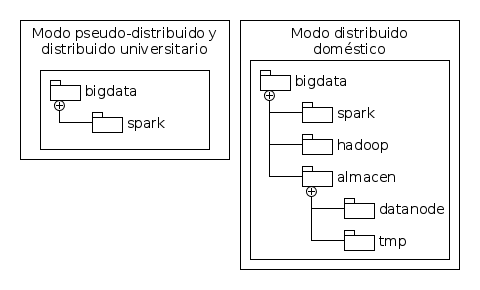
\includegraphics[scale=0.7]{diagramas/fichAntes}
\end{figure}

En este apartado explicaremos la estructuración realizada para establecer una organización clara y sencilla como se estableció en el apartado \ref{diseñoFich} del diseño.

Para ello, en el modo pseudo-distribuido y en el distribuido universitario se establecerá la estructura mostrada en la figura \ref{fig:fichSinRepli}. Para ello se crearán las siguientes carpetas:

\begin{itemize}
\item \textbf{/\$HOME/bigdata/almacen/data/unprocessed/:} donde se cargarán y almacenaran los archivos \gls{CSV} sin procesar.
\item \textbf{/\$HOME/bigdata/almacen/data/processed/:} donde se almacenarán los archivos limpiados y tratados por la arquitectura.
\item \textbf{/\$HOME/bigdata/almacen/results/:} donde se almacenarán los resultados.
\item \textbf{/\$HOME/bigdata/src/:} donde se alojará el código de los componentes del sistema.
\end{itemize}

\begin{figure}[htp!]
\centering
\caption{Estructura de los ficheros para los modos pseudo-distribuido y distribuido universitario}
\label{fig:fichSinRepli}
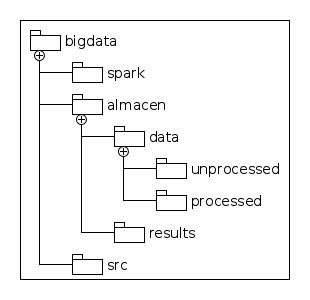
\includegraphics[scale=0.7]{diagramas/fichSinRepli}
\end{figure}

Con respecto al modo distribuido doméstico, al contar con las carpetas necesarias para la replicación de los datos, se establecerá la estructura de la figura \ref{fig:fichConRepli}. Para ello se crearán las siguientes carpetas:

\begin{itemize}
\item \textbf{/\$HOME/bigdata/almacen/results/:} donde se almacenarán los resultados.
\item \textbf{/\$HOME/bigdata/src/:} donde se alojará el código de los componentes del sistema.
\end{itemize}

\begin{figure}[htp!]
\centering
\caption{Estructura de los ficheros para el modos distribuido doméstico}
\label{fig:fichConRepli}
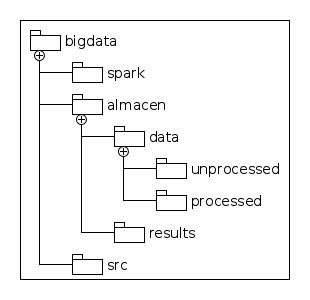
\includegraphics[scale=0.7]{diagramas/fichConRepli}
\end{figure}
 
Para crear las carpetas contenedoras de las trazas de los taxis, al estar estas contenidas dentro del sistema de replicación, será necesarias crearlas mediante los comandos del sistema de ficheros de \textit{Apache Hadoop}. En el fragmento de código \ref{mkdirHDFS} se muestran los comandos necesarios para crear las carpetas ``unprocessed'' y ``processed'' dentro del sistema de replicación.

\begin{lstlisting}[label=mkdirHDFS,language=sh,frame=single,caption=Comandos para crear las carpetas de datos en el \gls{HDFS}]
hdfs namenode -format
hdfs dfs -mkdir /unprocessed
hdfs dfs -mkdir /processed
\end{lstlisting}

Tras la creación de estas carpetas, ya tendremos la estructura de ficheros que la arquitectura utilizará para su funcionamiento.

\subsection{Establecimiento de los permisos para el modo distribuido doméstico}
Para evitar problemas de permisos en la lectura de ficheros, se creó en el apartado \ref{grupoComun}, en esta parte haremos efectiva la creación de este usuario, estableciendo al grupo permisos de lectura y escritura en la estructura de ficheros del sistema en todos los nodos que formen el clúster.

Para ello ejecutaremos el comando escrito en el fragmento de código \ref{permisos} que establecerá los permisos del grupo para la carpeta.

\begin{lstlisting}[label=permisos,language=sh,frame=single,caption=Comando para establecer permisos de lectura y escritura en el sistema de ficheros de la arquitectura]
sudo chown adrigrillo:spark -R /$HOME/bigdata/
\end{lstlisting}

\section{Obtención de las trazas de los taxis y ficheros sin procesar}
El fichero de datos con los viajes de los taxis de la Ciudad de Nueva York es un fichero \gls{CSV} de 33 \gls{GB}. Este fichero, a la fecha en la que se comenzó a trabajar en el proyecto, en febrero de 2017, se podía descargar desde la página de la competición \cite{grandChallenge}, obteniendo así un fichero llamado ``sorted\_data\_full.csv'' que contiene todos los viajes ordenadas por fecha.

Este fichero será introducido en la carpeta de datos sin procesar de la arquitectura y será renombrado a ``full.csv''. Además, a partir de dicho fichero, se crearán más, que sean fragmentos de menor tamaño que este siguiendo lo establecido en la tabla \ref{ficherosCSV}.

Para la creación de los ficheros parciales se utilizará el comando ``head'' de la terminal de Linux, al tratarse reducciones en base al número de registros del fichero original y, cada registro, ocupar una línea, mediante este comando se cogerá el número de líneas indicado desde la primera hasta tal línea y se guardará en el archivo.

\section{Carga de los ficheros en el sistema}
Para la carga de los ficheros creados en el paso anterior distinguiremos entre los dos sistemas de almacenamiento que hemos implementado. Por un lado, tenemos el modo pseudo-distribuido y el distribuido universitario que utilizan el sistema de ficheros del \gls{SO} y, por otro, el sistema distribuido doméstico que hace uso del \gls{HDFS}.

Para el primer grupo, la carga de los ficheros en el sistema se limita a la copia de estos dentro de la carpeta destinada a los ficheros sin procesar, ``/\$HOME/bigdata/almacen/data/unprocessed/''.

Para el modo distribuido, la carga de estos ficheros necesita de los comandos para la gestión del \gls{HDFS}, por tanto, para la carga de los ficheros se utilizará el comando del fragmento de código \ref{cargaFicheroHDFS}. Donde ``ficheroSinProcesar.csv'' será el nombre del fichero a cargar.

\begin{lstlisting}[label=cargaFicheroHDFS,language=sh,frame=single,caption=Comando para añadir los ficheros sin procesar al sistema de replicación]
hdfs dfs -put ficheroSinProcesar.csv unprocessed/
\end{lstlisting}

\section{Análisis y procesamiento de los datos \label{anaProcData}}
En este apartado se va a analizar el fichero de trazas de taxis y se va a describir el proceso de creación del componente de limpieza y tratamiento de los datos. Este componente será el mismo para todas las configuraciones de la arquitectura, es decir, el código será el mismo. Siendo la única diferencia la forma de acceder a los datos en el caso del modo distribuido doméstico.

El siguiente bloque representa un registro de un viaje en el fichero original descargado, que presenta la estructura que se puede apreciar en la tabla \ref{tab:trazaOrig}. 


\begin{verbatim}
07290D3599E7A0D62097A346EFCC1FB5,E7750A37CAB07D0DFF0AF7E3573AC141,
2013-01-01 00:00:00,2013-01-01 00:02:00,120,0.44,-73.956528,40.716976,
-73.962440,40.715008,CSH,3.50,0.50,0.50,0.00,0.00,4.50
\end{verbatim}

\begin{table}[htp!]
\centering
\caption{Campos de la traza de un viaje del fichero original}
\label{tab:trazaOrig}
\begin{tabular}{|l|l|}
\hline
\multicolumn{1}{|c|}{\textbf{NOMBRE}} & \multicolumn{1}{c|}{\textbf{SIGNIFICADO}}                  \\ \hline
medallon                              & Identificador md5sum del taxi                              \\ \hline
licencia                              & Identificador md5sum de la licencia del taxi               \\ \hline
hora\_subida                          & Hora a la que se sube el/la/los/las pasajero/a/os/as       \\ \hline
hora\_bajada                          & Hora a la que se baja el/la/los/las pasajero/a/os/as       \\ \hline
duracion\_viaje\_seg                  & Duración del viaje en segundos                             \\ \hline
distancia\_viaje                      & Distancia del viaje en millas                              \\ \hline
longitud\_subida                      & Coordinada de longitud de la subida                        \\ \hline
latitud\_subida                       & Coordinada de latitud de la subida                         \\ \hline
longitud\_bajada                      & Coordinada de longitud de la bajada                        \\ \hline
latitud\_bajada                       & Coordinada de latitud de la bajada                         \\ \hline
tipo\_pago                            & Método de pago (Tarjeta o efectivo)                        \\ \hline
tarifa                                & Cantidad de la tarifa en dólares                           \\ \hline
recargo                               & Cantidad del recargo en dólares                            \\ \hline
tasas                                 & Cantidad de las tasas en dólares                           \\ \hline
propina                               & Cantidad de la propina en dólares                          \\ \hline
peaje                                 & Cantidad de los peajes de los puentes o tuneles en dólares \\ \hline
cantidad\_total                       & Cantidad total en dólares                                  \\ \hline
\end{tabular}
\end{table}

Primeramente, para facilitar las operaciones posteriormente al trabajar con \textit{Apache Spark}, se establecerá el esquema de la tabla, es decir, los nombres de las columnas expuestos en la tabla \ref{tab:trazaOrig} debido a que los \gls{CSV} aportados no contienen cabeceras. Esto nos permitirá acceder a los atributos de la traza con el nombre a los datos. Para ello, utilizaremos el código escrito en el fragmento \ref{inferSchema}

\begin{lstlisting}[label=inferSchema,language=Python,frame=single,caption=Código para establecer el esquema del \gls{CSV} y facilitar el acceso a los atributos]
nombreColumnas = 
StructType([StructField("medallon", StringType(), True),
StructField("licencia", StringType(), True),
StructField("hora_subida", TimestampType(), True),
StructField("hora_bajada", TimestampType(), True),
StructField("duracion_viaje_seg", IntegerType(), True),
StructField("distancia_viaje", DecimalType(precision=10, scale=2), True),
StructField("longitud_subida", DecimalType(precision=18, scale=14), True),
StructField("latitud_subida", DecimalType(precision=18, scale=14), True),
StructField("longitud_bajada", DecimalType(precision=18, scale=14), True),
StructField("latitud_bajada", DecimalType(precision=18, scale=14), True),
StructField("tipo_pago", StringType(), True),
StructField("tarifa", DecimalType(precision=10, scale=2), True),
StructField("recargo", DecimalType(precision=10, scale=2), True),
StructField("tasas", DecimalType(precision=10, scale=2), True),
StructField("propina", DecimalType(precision=10, scale=2), True),
StructField("peaje", DecimalType(precision=10, scale=2), True),
StructField("cantidad_total", DecimalType(precision=10, scale=2), True)])
\end{lstlisting}

Una vez creado el esquema, este será utilizado en la lectura de los ficheros, al establecerlo como argumento de la función \textit{read}. Por otro lado, para la correcta lectura y trabajo con las fechas, en la misma función, habrá que indicar correctamente el formato de la misma, que en este caso será un string del tipo ``"yyyy-MM-dd HH:mm:ss". Esto nos permitirá la transformación de las fechas en \textit{timestamps} con los que trabajar de forma más cómoda al poder obtener los días de la semana a partir de la fecha o poder sumar y restar en horas, minutos y segundos.

\begin{lstlisting}[label=readCSV,language=python,frame=single,caption=Código para leer los ficheros \gls{CSV}]
""" Lectura de ficheros para los modos pseudo-distribuido
     y distribuido universitario """
data = spark.read.csv("/$HOME/bigdata/almacen/data/unprocessed/nombreFichero.csv", schema=nombreColumnas, timestampFormat="yyyy-MM-dd HH:mm:ss")

""" Lectura de ficheros para el modo distribuido domestico """
data = spark.read.csv("hdfs://master:9000/unprocessed/nombreFichero.csv", schema=nombreColumnas, timestampFormat="yyyy-MM-dd HH:mm:ss")
\end{lstlisting}

En el fragmento de código \ref{readCSV} se encuentra la forma usada para leer los archivos por \textit{Apache Spark} para los dos tipos de almacenamiento que podemos encontrar en el sistema dependiendo de la configuración utilizada.

El primer paso tras introducir los datos en el sistema y ser leídos, es limpiar aquellos registros que no son válidos. En este caso, a parte de los registros que son nulos, debido a que los datos se hayan recogido de forma inválida, la organización del concurso establece un límite de coordenadas para contar el viaje como válido. Es decir, entre las trazas puede haber algún registro cuyas coordenadas se salgan del límite de la ciudad de Nueva York, siendo este inválido. Las coordenadas que limitan el área son:

\begin{itemize}
\item Latitud inicial = 41.477182778
\item Longitud inicial = -74.916578
\item Latitud final = 40,129715978
\item Longitud final = -73.120778
\end{itemize}

Por otro lado, dentro de las trazas existen atributos que no aportan información útil para los posteriores cálculos, atributos como ``distancia\_viaje'', ``recargo'', ``tasas'' o ``peaje''. Estos serán eliminados de todos los registros, ya que, como se va a pasar a un tipo de almacenamiento columnar tras el procesamiento de los datos, es decir, los datos serán guardados en archivos \textit{.parquet}, estos atributos supondrían un gasto en espacio innecesario, ahorrándolo con su supresión.

Por tanto, para la limpieza de los ficheros, aparte de borrar los atributos indicados, se suprimirán los registros en los siguientes casos:

\begin{itemize}
\item Cuando el ID del taxi o de la licencia es nulo.
\item Cuando las horas de subida y bajada coinciden.
\item Cuando la duración del viaje sea igual a 0.
\item Cuando el tipo de pago es diferente a: en efectivo o con tarjeta.
\item Cuando el precio total es igual a 0.
\item Cuando las posiciones de inicio y final son las mismas.
\item Cuando alguna coordenada de posición no esté dentro de los límites de las coordenadas indicadas anteriormente.
\end{itemize}

Debido a la versatilidad de \textit{Apache Spark}, este permite usar lenguaje \gls{SQL} para trabajar con los datos, así como métodos propios. Por tanto, para la limpieza de los datos, realizaremos dos consultas, una para controlar los límites de coordenadas, que utilizará los métodos propios del \gls{framework} para el filtrado debido a la posibilidad de uso de variables globales para usar comparaciones y, otra, que hará el filtrado de las demás condiciones que invalidan un registro, que será en lenguaje \gls{SQL}.

Por tanto, en el fragmento de código \ref{filtroSQL} podemos encontrar la consulta que filtra la mayoría de condiciones y, en el fragmento \ref{filtroLim}, el código que filtra los registros que no están dentro de los límites establecidos.

Una vez realizada la limpieza de los registros, el siguiente paso es hacer el tratamiento de los datos para ajustarse a los requisitos establecidos por la competición. Estos requisitos implican la creación de una cuadrícula con la que dividir la ciudad de Nueva York y poder hacer cálculos desde ella, en vez de usar las coordenadas del fichero original.

Esta cuadrícula tendrá celdas de 500x500 metros y estará compuesta por 300 celdas de ancho por 300 de alto, suponiendo una extensión de 150 kilómetros al este y 150 kilómetros al sur. Para establecer la cuadrícula se da el centro de la primera celda, en la parte superior izquierda, en coordenadas y, a partir de ahí, se establece el resto.

El proceso para la obtención de las coordenadas de cada celda de la cuadrícula se puede encontrar en el anexo \ref{cuadricula}. Sin embargo, para el procesamiento de estos datos, lo que nos interesa es obtener las cuadrículas a la que pertenece cada registro, es decir, a partir de las latitudes y longitudes de subida y bajada del registro, obtener las cuadrículas $(x, y)$ de subida y bajada, pudiendo ser utilizadas para las consultas.

\clearpage
\begin{lstlisting}[label=filtroSQL,language=SQL,frame=single,caption=Filtro de registros en \gls{SQL} para registros inválidos]
SELECT 
    medallon,
    licencia,
    hora_subida,
    hora_bajada,
    duracion_viaje_seg,
    longitud_subida,
    latitud_subida,
    longitud_bajada,
    latitud_bajada,
    tipo_pago,
    tarifa,
    propina,
    cantidad_total
FROM unprocessed 
WHERE   
    medallon <> '' AND 
    licencia <> '' AND
    hora_subida <> hora_bajada AND
    duracion_viaje_seg > 0 AND
    cantidad_total > 0 AND
    longitud_subida <> longitud_bajada AND
    latitud_subida <> latitud_bajada AND
    (tipo_pago == 'CHS' OR tipo_pago == 'CRD')
\end{lstlisting}

\begin{lstlisting}[label=filtroLim,language=python,frame=single,caption=Filtro de coordenadas para los registros que sobrepasan el límite]
data = data.where(data.longitud_subida >= INITIAL_LONGITUDE) \
    .where(data.longitud_subida <= FINAL_LONGITUDE) \
    .where(data.longitud_bajada >= INITIAL_LONGITUDE) \
    .where(data.longitud_bajada <= FINAL_LONGITUDE) \
    .where(data.latitud_subida >= FINAL_LATITUDE) \
    .where(data.latitud_subida <= INITIAL_LATITUDE) \
    .where(data.latitud_bajada >= FINAL_LATITUDE) \
    .where(data.latitud_bajada <= INITIAL_LATITUDE)
\end{lstlisting}

Por tanto, para ello, en los registros se crearán cuatro nuevos atributos, donde se calculará la cuadrícula a partir de las coordenadas. Estos serán:

\begin{itemize}
\item \textbf{cuad\_latitud\_subida:} Que será el valor $x$ de la cuadrícula para la posición de subida del viaje.
\item \textbf{cuad\_longitud\_subida:} Que será el valor $y$ de la cuadrícula para la posición de subida del viaje.
\item \textbf{cuad\_latitud\_bajada:} Que será el valor $x$ de la cuadrícula para la posición de bajada del viaje.
\item \textbf{cuad\_longitud\_bajada:} Que será el valor $y$ de la cuadrícula para la posición de bajada del viaje.
\end{itemize}

Los cálculos de la celda a la que pertenece una coordenada se realiza con las siguientes fórmulas, donde ``INITIAL\_LATITUDE'' e ``INITIAL\_LONGITUDE'' son las coordenadas iniciales de latitud y longitud de la cuadrícula y ``LATITUDE'' y ``LONGITUDE'' son el tamaño de una celda en coordenadas. Las fórmulas son:

\begin{verbatim}
Cuadrícula de latitud =
= int(floor((INITIAL_LATITUDE - latitud_subida)/LATITUDE)) + 1 

Cuadrícula de longitud = 
= int(floor(abs(INITIAL_LONGITUDE - longitud_dada)/LONGITUDE)) + 1
\end{verbatim}

Por otro lado, como en el diseño de las consultas, en el apartado \ref{disConsultas}, se diseñaron dos modificaciones de las originales donde se tenía en cuenta el día de la semana para realizar los cálculos. Esto planteaba dos posibilidades para la implementación, realizar el cálculo del día en la ejecución de la consulta, que implicaría añadir el número de cálculos en cada consulta y cada ejecución, o crear un nuevo atributo en el registro que indicase el día de la semana del viaje, realizando el cálculo una única vez durante el procesamiento y limpieza de los ficheros.

Debido al ahorro en cálculos que esta segunda opción suponía, se tomó este camino, por lo que se crea un nuevo atributo llamado ``dia\_semana''. Para ello se crea una función de usuario para que \textit{Apache Spark} pueda procesar los registros y establecer el resultado de esta en el atributo, esta función se muestra en el código \ref{diaSemana}.

\begin{lstlisting}[label=diaSemana,language=Python,frame=single,caption=Función día de la semana para crear nuevo atributo]
def dia_fecha(fecha):
    return fecha.weekday()

calcular_dia = udf(dia_fecha, IntegerType())
\end{lstlisting}

Por último, tras el tratamiento de los ficheros, el paso final es el guardado de estos ficheros. Para ello, como se ha comentado anteriormente, utilizaremos \textit{Apache Parquet} como formato y \textit{Snappy} como sistema de compresión de los mismos. Esto nos permitirá un ahorro de espacio elevado y una velocidad de procesamiento mayor que utilizando los ficheros \gls{CSV}, como se comprueba en los apartados \ref{compFichDatos} y \ref{resCompFich}.

El almacenamiento se hará en la carpeta ``processed'' de la arquitectura, manteniendo el nombre del fichero original del \gls{CSV}. En el fragmento de código \ref{tratyguardado}, se encuentra el tratamiento de los datos, añadiendo los atributos de la cuadrícula y el día de la semana, y el guardado del fichero resultante.

\clearpage
\begin{lstlisting}[label=tratyguardado,language=Python,frame=single,caption=Código para el tratamiento y guardado del fichero procesado]
""" Establecemos el sistema de cuadriculas y 
calculamos el dia de la semana """
data = data.withColumn("cuad_latitud_subida", floor((INITIAL_LATITUDE - data.latitud_subida)/LATITUDE) + 1) \
    .withColumn("cuad_longitud_subida", floor(abs(INITIAL_LONGITUDE - data.longitud_subida)/LONGITUDE) + 1) \
    .withColumn("cuad_latitud_bajada", floor((INITIAL_LATITUDE - data.latitud_bajada)/LATITUDE) + 1) \
    .withColumn("cuad_longitud_bajada", floor(abs(INITIAL_LONGITUDE - data.longitud_bajada)/LONGITUDE) + 1) \
    .withColumn("dia_semana", CALCULAR_DIA(data.hora_subida))

""" Guardado del fichero en sistema pseudo-distribuido y
	 distribuido universitario """
data.write.option("compression", "snappy") \
        .parquet("/$HOME/bigdata/almacen/data/processed/" + nombre + ".parquet")

""" Guardado del fichero en sistema distribuido domestico """
data.write.option("compression", "snappy") \
        .parquet("hdfs://master:9000/processed/" + nombre + ".parquet")
\end{lstlisting}

\section{Implementación de las consultas \label{impConsultas}}
Como se estableció en el diseño de la arquitectura, apartado \ref{disConsultas}, se establecieron cuatro consultas que el sistema sería capaz de realizar sobre los datos. Dos sobre las rutas más frecuentes y dos sobre las zonas que más beneficios aportarían a los taxistas si iniciasen un viaje desde allí, ambos tipos tienen una consulta donde se tiene en cuenta la estacionalidad y otra donde no.

Estas consultas utilizarán los datos ya procesados anteriormente y que residirán en la carpeta ``processed'', por lo que el primer argumento de todas estas consultas será indicar el fichero sobre el que se trabajará. El resto de argumentos dependerán de la consulta. Tras analizar los datos, el resultado será almacenado en un fichero con el nombre de la consulta, en la carpeta ``results'', donde, aparte del resultado obtenido, se guardará el tiempo de ejecución, que será lo más importante para analizar el sistema posteriormente.

\subsection{Rutas más frecuentes sin estacionalidad \label{freqSinExplicacion}}
El objetivo de esta consulta es obtener las diez rutas más frecuentes durante los 30 minutos anteriores a una fecha y hora establecidas por el usuario, que será el argumento de la consulta. Estas rutas serán válidas únicamente si el viaje ha sido completado, es decir, si el usuario se ha bajado del taxi dentro de la franja del tiempo. 

Por tanto, esta consulta consistirá en dos acciones sobre los datos. Primero, se deberá filtrar los resultados que cumplan con la condición de tiempo, es decir, que hayan acabado dentro de la franja horaria. Posteriormente, se realizará una agrupación por las coordenadas de subida y de bajada y conteo respecto a esta. Es decir, los registros se agruparan en conjuntos que tengan las mismas coordenadas de la cuadrícula de subida y bajada y se contará el número de elementos en cada grupo.

Finalmente, se tomarán los 10 grupos con más registros, y se ordenarán de mayor a menor. El código de la consulta se puede encontrar en el fragmento \ref{codFreq} y la salida de la consulta será la siguiente:

\begin{verbatim}
fecha_subida, fecha_bajada, 0: (celda_subida) (celda_bajada),
1: (celda_subida) (celda_bajada), ..., 9: (celda_subida) (celda_bajada),
tiempo_ejecucion
\end{verbatim}

\begin{lstlisting}[label=codFreq,language=Python,frame=single,caption=Consulta diez rutas más frecuentes]
frequent = data.filter(data.hora_subida <= tiempo_fin) \
        .filter(data.hora_subida >= tiempo_inicio) \
        .filter(data.hora_bajada <= tiempo_fin) \
        .filter(data.hora_bajada >= tiempo_inicio) \
        .groupBy("cuad_longitud_subida", "cuad_latitud_subida", "cuad_longitud_bajada", "cuad_latitud_bajada") \
        .count().orderBy("count", ascending=False)
frequent = frequent.take(10)
\end{lstlisting}

\subsection{Rutas más frecuentes con estacionalidad}
Esta consulta, que es una modificación de la anterior, busca también las diez rutas más frecuentes, pero tiene en cuenta la estacionalidad, es decir, tiene en cuenta el mes en el que se realiza la consulta. Para ello, el usuario introducirá como argumentos el mes, el día de la semana y la hora en la que quiere realizar la consulta.

El sistema, al igual que en la anterior, tomará los viajes que acaben en la media hora anterior a la hora dada, los días de la semana señalados. Además dará un valor mayor a los viajes cercanos al mes indicado y su anterior. Posteriormente, los agrupará por celda de subida y bajada, sumando el valor de la relevancia del viaje y ordenará de mayor a menor con respecto al valor de la misma, devolviendo las diez rutas que mayor valor tengan en el atributo relevancia.

La relevancia de un viaje es 1 por defecto, para simular el valor que tendría en un \textit{count}, sin embargo, si el registro es cercano al mes indicado, pasará a doblar su valor de relevancia, es decir, 2. Un registro es cercano si se encuentra 30 días antes o después del primer día del mes indicado.

Para el funcionamiento de esta consulta se deben crear dos funciones de usuario para que \textit{Apache Spark} pueda utilizarlas en el filtrado de datos, estas serán las que se encuentran en el fragmento \ref{udfFreq}.

\begin{lstlisting}[label=udfFreq,language=Python,frame=single,caption=Funciones de usuario para filtrado de la consulta de rutas frecuentes con estacionalidad]
def comparar_hora(hora):
    """
        Metodo que filtra las horas de los registros para que 
        concuerden con las horas de busqueda deseada
        :param hora: Timestamp completo
        :return: True si las horas del timestamp estan entre las deseadas
        False si lo contrario
    """
    if hora.time() <= HORA_FIN.time() and hora.time() >= HORA_INICIO.time():
        return True
    return False

def relevancia(fecha):
    """
        Metodo que da mas relevancia a los viajes mas cercanos
        a la fecha de busqueda deseada.
        Si la diferencia es menor a un mes de la fecha
        dada los registros tienen mas relevancia
        :param fecha: Timestamp completo
        :return: 2 si el viaje esta cerca de la fecha deseada, 1 si no
    """
    diferencia = fecha - HORA_FIN
    if diferencia < timedelta(days=30) and diferencia > timedelta(days=-30):
        return 2
    else:
        return 1

comprobar_hora = udf(comparar_hora, BooleanType())
calcular_relevancia = udf(relevancia, IntegerType())
\end{lstlisting}

\clearpage
Tras declarar estás funciones, el código de la consulta se puede encontrar en el fragmento \ref{codFreqDay}.

\begin{lstlisting}[label=codFreqDay,language=Python,frame=single,caption=Código consulta de diez rutas más frecuentes teniendo en cuenta la estacionalidad]
""" Devuelve el integer del dia de la semana para filtrar
	 posteriormente los dias que no coinciden con este """
dia_elegido = obtener_dia_semana(DIA_SEMANA)

""" Filtramos los datos con respecto al dia de la semana 
    y la hora.
    Ademas le damos un relevancia a cada viaje
    para el posterior count """
filtered = data.filter(data.dia_semana == dia_elegido) \
	.withColumn("filtroSubida", comprobar_hora(data.hora_subida)) \
	.withColumn("filtroBajada", comprobar_hora(data.hora_bajada)) \
	.withColumn('relevancia', calcular_relevancia(data.hora_subida))

filtered = filtered.filter(filtered.filtroSubida == True) \
    .filter(filtered.filtroBajada == True)

""" Agrupamos por rutas y hacemos el recuento de viajes """
frequent = filtered.groupBy("cuad_longitud_subida", "cuad_latitud_subida", "cuad_longitud_bajada", "cuad_latitud_bajada") \
    .sum("relevancia") \
    .select(col("cuad_longitud_subida"), col("cuad_latitud_subida"), col("cuad_longitud_bajada"), col("cuad_latitud_bajada"), col("sum(relevancia)").alias("frecuencia")) \
    .orderBy("frecuencia", ascending=False)

final = frequent.take(10)
\end{lstlisting}

La salida de esta consulta será muy parecida a la anterior, indicando solo la hora de subida y bajada, siendo la siguiente.

\begin{verbatim}
hora_subida, hora_bajada, 0: (celda_subida) (celda_bajada),
1: (celda_subida) (celda_bajada), ..., 9: (celda_subida) (celda_bajada),
tiempo_ejecucion
\end{verbatim}

\subsection{Zonas que más beneficios proporcionarían al taxista sin estacionalidad \label{profSinExplicacion}}
En esta consulta se busca conseguir las diez zonas, celdas de la cuadrícula, donde el taxista obtendría mayor beneficio empezando un viaje en dicha zona. Para ello, el usuario introducirá como argumento la fecha y la hora sobre la que quiere hacerse la consulta.

El beneficio de una zona se obtiene dividiendo el beneficio obtenido por los taxistas en el conjunto de viajes empezados en dicha zona durante los últimos 15 minutos por la cantidad de taxis vacíos que hay en la zona.

El beneficio que obtiene el taxista con un viaje es la suma de la tarifa y la propina del mismo. Por tanto, el beneficio de una zona, será la media del beneficio de los viajes que han acabado en los últimos 15 minutos y empezaron en esa zona. 

Por tanto, esta consulta se realizará en dos partes, por un lado, se obtendrán el número de taxis libres y, por otro, los beneficios de los taxistas. Posteriormente se unirán los resultados y se realizarán los cálculos para obtener los datos finales y, por tanto, las zonas con más beneficios. La fórmula a aplicar es la siguiente:

\begin{center}
$Beneficio \; zona = \dfrac{media \; de \; tarifa + propina \; (15 \; min)}{taxis \; vacios \; en \; zona \; (30 \; min)}$
\end{center}

\subsubsection{Taxis vacíos en las zonas}
El código de este proceso de la consulta se puede encontrar en el fragmento \ref{taxisVacios}, cuya técnica para obtener los taxis vacíos en una zona durante la última media hora es la siguiente: 

\begin{enumerate}
\item Se obtienen los viajes de subida y bajada de los taxis en la última media hora.

\item Se procede a juntar ambos conjuntos de datos mediante un \textit{join} donde solo los taxis vacíos puedan crear una fila de la tabla. De esta forma se puede comprobar que no se tienen en cuenta los taxis que hayan sido cogidos de nuevo.

\item De esta lista, se eliminan los taxis que hayan sido cogidos tras la ultima bajada, es decir, que hayan iniciado otro viaje durante la ventana de tiempo y no lo haya finalizado.
\end{enumerate}

\clearpage
\begin{lstlisting}[label=taxisVacios,language=Python,frame=single,caption=Código para obtener los taxis vacíos en las zonas de la ciudad durante la última media hora]
# Obtenemos los ultimos viajes de subida y bajada de los taxis
bajadas30 = tripsDown \
    .select("medallon", "hora_bajada", "cuad_latitud_bajada", "cuad_longitud_bajada") \
    .orderBy("hora_bajada", ascending=False) \
    .dropDuplicates(subset=["medallon"])

subidas30 = tripsUp \
    .select("medallon", "hora_subida").orderBy("hora_subida", ascending=False) \
    .dropDuplicates(subset=["medallon"]).withColumnRenamed("medallon", "taxi")

""" Procedemos a juntar ambos conjuntos de datos para asi
    poder comprobar que no se tienen en cuenta los taxis
    que hayan sido cogidos de nuevo """
# Spark falla join si el nombre de la columna es el mismo,
# renombrado a taxi
joined = bajadas30.join(subidas30, bajadas30.medallon == subidas30.taxi, "leftouter") \
    .select("medallon", "hora_bajada", "hora_subida", "cuad_latitud_bajada", "cuad_longitud_bajada")

# Eliminamos los taxis que hayan sido cogidos tras la ultima bajada
estado_taxis = joined.select(joined.medallon, joined.cuad_latitud_bajada, joined.cuad_longitud_bajada, when(joined.hora_subida > joined.hora_bajada, 1).otherwise(0).alias("taxi_ocupado"))
    
taxis_filtrados = estado_taxis.filter(estado_taxis.taxi_ocupado == 0)

taxis_libres = taxis_filtrados.groupBy("cuad_latitud_bajada", "cuad_longitud_bajada").count() \
   .select(col("cuad_latitud_bajada"), col("cuad_longitud_bajada"), col("count").alias("taxis_libres"))
\end{lstlisting}

\clearpage
\subsubsection{Beneficio de las zonas}
El código de este fragmento se puede encontrar en el fragmento \ref{beneficioZona}. Para obtener estos datos, los pasos a seguir son los siguientes:

\begin{enumerate}
\item Se realiza un filtrado tomando los viajes acabados en los últimos 15 minutos.
\item Estos viajes son agrupados por la celda en la que son iniciados.
\item Se calcula la media de la tarifa y de la propina de cada zona establecida en el agrupamiento.
\item Se realiza la suma de la media de la tarifa y de la propina para cada zona, obteniéndose así el beneficio medio de las zonas.
\end{enumerate}

\begin{lstlisting}[label=beneficioZona,language=Python,frame=single,caption=Código para obtener el beneficio de las zonas de la ciudad durante los últimos quince minutos]
beneficios = trips15.groupBy("cuad_latitud_subida", "cuad_longitud_subida") \
    .avg("tarifa", "propina") \
    .select(col("cuad_latitud_subida"), col("cuad_longitud_subida"), \ col("avg(tarifa)") + col("avg(propina)")).alias("beneficios"))
\end{lstlisting}

\subsubsection{Obtención del beneficio proporcionado para el taxista}
Tras obtener los datos necesarios para obtener el beneficio real de la zona, el siguiente paso es unirlos y operar sobre ellos. Para ello, lo primero es realizar el \textit{join} de las dos tablas. En este caso, la única tabla que creará filas será la tabla de beneficio medio de las zonas, debido a que nos interesa evitar los cálculos de zonas donde no hay datos de beneficio pero existen taxis libres.

Tras la unión de estas dos tablas, se creará un nuevo atributo, llamado ``beneficio'' que será el resultado de la división del beneficio medio de la zona entre el número de taxis libres en dicha zona. Para evitar las divisiones por 0 cuando no hay taxis libres en la zona, se ha sumado 1 a la cuenta de los taxis libres. De esta forma, cuando no hay taxis se obtiene el beneficio integro de la zona y cuando hay algún taxista, se obtiene la repartición de beneficios.

La salida de esta consulta serán las diez zonas que más beneficios aportarían al taxista durante la ventana de tiempo introducida. Esta será la siguiente:

\begin{verbatim}
fecha_subida, fecha_bajada, 0: (celda_zona), 1: (celda_zona), ..., 
9: (celda_zona), tiempo_ejecucion
\end{verbatim}

El código de la unión de estas dos tablas y obtención de los resultados es el escrito en el fragmento \ref{unioProfi}.

\begin{lstlisting}[label=unioProfi,language=Python,frame=single,caption=Código de la unión de tablas de beneficios y taxis libres y obtención de los resultados de la consulta]
condicion = [beneficios.cuad_latitud_subida == taxis_libres.cuad_latitud_bajada, beneficios.cuad_longitud_subida == taxis_libres.cuad_longitud_bajada]

profitable = beneficios \
    .join(taxis_libres, condicion, "leftouter") \
    .select(col("cuad_latitud_subida").alias("cuad_latitud"), col("cuad_longitud_subida").alias("cuad_longitud"), (col("beneficios") / when(taxis_libres.taxis_libres > 0, (taxis_libres.taxis_libres + 1)).otherwise(1)).alias("beneficio")) \
    .orderBy("beneficio", ascending=False)

profitable = profitable.take(10)
\end{lstlisting}

\subsection{Zonas que más beneficios proporcionarían al taxista con estacionalidad}
Esta consulta que es una modificación de la anterior, tiene el mismo objetivo que esta, obtener las diez zonas que más beneficios puede procurar al taxista. En esta, como en el caso de las rutas frecuentes con estacionalidad, tiene en cuenta el mes introducido para obtener los resultados.

Por tanto, el usuario introducirá como argumentos el mes, el día de la semana y la hora en la que quiere realizar la consulta. El sistema, realizará los mismos cálculos que la consulta original, sin embargo, la diferencia está en que se aplicará un factor de influencia a los registros dependiendo de la cercanía de la fecha del registro al mes deseado por el usuario.

Este factor de influencia se utilizará tanto sobre el número de taxis libres como el valor de los beneficios medios de las zonas. Este factor se aplicará mediante la creación de una función de usuario de \textit{Apache Spark}, escrito en el fragmento de código \ref{infProf}.

Además, al no utilizar \textit{timestamps} completos en esta consulta, también se han de crear dos funciones de usuario para filtrar los registros por tiempo. Estas serán las escritas en el código \ref{ufTiempo}.

\clearpage
\begin{lstlisting}[label=infProf,language=Python,frame=single,caption=Función de usuario para aplicar el factor de relevancia]
def relevancia(fecha):
    """
        Metodo que da mas relevancia a los viajes mas cercanos
        a la fecha de busqueda deseada.
        Si la diferencia es menor a un mes de la fecha
        dada los registros tienen mas relevancia
        :param fecha: Timestamp completo
        :return: 2 si el viaje esta cerca de la fecha deseada, 1 si no
    """
    diferencia = fecha - HORA_FIN
    if diferencia < timedelta(days=7) and diferencia > timedelta(days=-7):
        return 1.0
    elif diferencia < timedelta(days=14) and diferencia > timedelta(days=-14):
        return 0.75
    elif diferencia < timedelta(days=21) and diferencia > timedelta(days=-21):
        return 0.5
    elif diferencia < timedelta(days=-28) and diferencia > timedelta(days=-28):
        return 0.25
    else:
        return 0

calcular_relevancia = udf(relevancia, FloatType())
\end{lstlisting}

\begin{lstlisting}[label=ufTiempo,language=Python,frame=single,caption=Funciones de usuario para filtrar los registros por tiempo]
def comparar_media_hora(hora):
    """
        Metodo que filtra las horas de los registros para que concuerden
        con las horas de busqueda deseada
        :param hora: Timestamp completo
        :return: True si las horas del timestamp estan entre las deseadas
        False si lo contrario
    """
    if hora.time() <= HORA_FIN.time() and hora.time() >= HORA_30.time():
        return True
    return False


def comparar_cuarto_hora(hora):
    """
        Metodo que filtra las horas de los registros para que concuerden
        con las horas de busqueda deseada
        :param hora: Timestamp completo
        :return: True si las horas del timestamp estan entre las deseadas
        False si lo contrario
    """
    if hora.time() <= HORA_FIN.time() and hora.time() >= HORA_15.time():
        return True
    return False

comprobar_media_hora = udf(comparar_media_hora, BooleanType())
comprobar_cuarto_hora = udf(comparar_cuarto_hora, BooleanType())
\end{lstlisting}

El código de esta consulta es el escrito en el fragmento de código \ref{codProfDay}. La salida de esta consulta serán las diez zonas que más beneficios aportarían al taxista durante la ventana de tiempo introducida, en el día de la semana introducido. Esta será la siguiente:

\begin{verbatim}
hora_subida, hora_bajada, 0: (celda_zona), 1: (celda_zona), ..., 
9: (celda_zona), tiempo_ejecucion
\end{verbatim}

\begin{lstlisting}[label=codProfDay,language=Python,frame=single,caption=Código de la consulta para obtener las diez zonas que proporcionan más beneficios al taxista teniendo en cuenta la estacionalidad]
dia_elegido = obtener_dia_semana(DIA_SEMANA)

# Filtramos los datos con respecto al dia de la semana y la hora
trips_down = data.filter(data.dia_semana == dia_elegido) \
    .filter(comprobar_media_hora(data.hora_bajada))

trips_up = data.filter(data.dia_semana == dia_elegido) \
    .filter(comprobar_media_hora(data.hora_subida))

# Borramos duplicados y los ordenamos por proximidad 
# a la hora deseada
down_30_min = trips_down.select("medallon", "hora_bajada", "cuad_latitud_bajada", "cuad_longitud_bajada") \
    .orderBy("hora_bajada", ascending=False) \
    .dropDuplicates(subset=["medallon"])



up_30_min = trips_up.select("medallon", "hora_subida").orderBy("hora_subida", ascending=False) \
    .dropDuplicates(subset=["medallon"]).withColumnRenamed("medallon", "taxi")

# spark falla join si el nombre de la columna es el mismo,
# renombrado a taxi
joined = down_30_min.join(up_30_min, down_30_min.medallon == up_30_min.taxi, "leftouter") \
    .select("medallon", "hora_bajada", "hora_subida", "cuad_latitud_bajada", "cuad_longitud_bajada")

# Sacamos los taxis que estan libres con su posicion
estado_taxis = joined.select(joined.medallon, joined.cuad_latitud_bajada, joined.cuad_longitud_bajada, joined.hora_bajada, when(joined.hora_subida > joined.hora_bajada, 1).otherwise(0).alias("taxi_ocupado"))

# Anyadimos el factor de influencia a cada taxi
# segun la distancia a fecha del registro
taxis_filtrados = estado_taxis.filter(estado_taxis.taxi_ocupado == 0) \
    .withColumn("influencia", calcular_relevancia(estado_taxis.hora_bajada))

# Calculamos el numero de taxis vacios en las zonas
taxis_libres = taxis_filtrados.groupBy("cuad_latitud_bajada", "cuad_longitud_bajada").count() \
    .select(col("cuad_latitud_bajada"), col("cuad_longitud_bajada"), col("count").alias("taxis_libres"))

# Calculamos la influencia de la zona con la media
# de la influencia de los taxis en dicha zona
influencia_taxis_libres = taxis_filtrados \
    .groupBy("cuad_latitud_bajada", "cuad_longitud_bajada") \
    .avg("influencia") \
    .select(col("cuad_latitud_bajada").alias("latitud"), col("cuad_longitud_bajada").alias("longitud"), col("avg(influencia)").alias("influencia"))

""" Calculamos la proporcion de taxis libres por zona, 
    esta proporcion es el numero de taxis libres en la 
    zona por la influencia de estos taxis.
    Siendo menos influyentes cuanto mas alejados
    en el tiempo """
condition = [taxis_libres.cuad_latitud_bajada == influencia_taxis_libres.latitud, taxis_libres.cuad_longitud_bajada == influencia_taxis_libres.longitud]

taxis_libres_prop = taxis_libres.join(influencia_taxis_libres, condition) \
    .select(col("cuad_latitud_bajada"), col("cuad_longitud_bajada"), round(col("taxis_libres") * col("influencia")).alias("proporcion_taxis_libres"))

"""
    PASAMOS A LOS BENEFICIOS
"""
# Filtramos viajes por tiempo y anyadimos influencia con
# respecto a la fecha deseada
trips_15 = trips_down.filter(comprobar_cuarto_hora(data.hora_bajada)) \
    .withColumn("influencia", calcular_relevancia(estado_taxis.hora_bajada))

# Obtenemos los beneficios de la zona con la influencia
# tenida en cuenta
beneficios = trips_15.groupBy("cuad_latitud_subida", "cuad_longitud_subida") \
    .avg("tarifa", "propina", "influencia") \
    .select(col("cuad_latitud_subida"), col("cuad_longitud_subida"), col("avg(tarifa)") + col("avg(propina)")) * col("avg(influencia)")).alias("beneficios"))

# Unimos los beneficios con los taxis libres y dividimo
# beneficios/taxis_libres
condicion = [beneficios.cuad_latitud_subida == taxis_libres.cuad_latitud_bajada, beneficios.cuad_longitud_subida == taxis_libres.cuad_longitud_bajada]

profitable = beneficios.join(taxis_libres_prop, condicion, "leftouter") \
    .select(col("cuad_latitud_subida").alias("cuad_latitud"), col("cuad_longitud_subida").alias("cuad_longitud"), col("beneficios") / col("proporcion_taxis_libres")).alias("beneficio")) \
    .orderBy("beneficio", ascending=False)

# Obtenemos el top 10
profitable = profitable.take(10)
\end{lstlisting}
